\chapter{基于ECL--SOA的DAS发射链路与DAS一体化收发模组}

\section{引言}

第二章从相干瑞利后向散射、集成SOA的ECL激光器脉冲发射、AOM移频、外差平衡探测和数字相位解调等方面建立了DAS系统的理论基础。要将上述原理落实为可稳定运行的实验系统，还需要解决发射光脉冲的功率与消光、移频窗口的时序匹配、收发光路的损耗与串扰以及多器件集成后的稳定性等工程问题。尤其对于采用集成SOA的ECL激光器的无EDFA发射链路，SOA既参与光功率放大，又参与脉冲形成，其驱动状态会同时作用于输出功率、脉冲波形、关断漏光、ASE噪声和外差拍频质量。因此，有必要从完整链路而非单一器件指标出发，对其工作特性和适用范围进行系统表征。

在该发射链路中，SOA与AOM、数据采集系统之间还存在不可忽略的动态时序关系。SOA载流子的建立与恢复、AOM声场的传播与稳定以及DAQ触发和采样窗口均具有有限响应时间。若三者仅采用相同命令边沿进行简单同步，有效光脉冲可能与AOM稳定衍射窗口或采集窗口不能充分重合，进而影响脉冲完整性、拍频信噪比和相位解调稳定性。另一方面，SOA工作状态变化与实测拍频变化之间可能同时受到器件动态、AOM支路、光路时延、温度和频谱分析窗口等因素影响。因而，本章将通过受控变量和对照实验逐项分离各因素的影响，在量化各支路贡献的基础上，判别SOA瞬态啁啾对拍频变化的具体作用。

为进一步降低分立光路中器件连接、重复装调和环境扰动带来的不确定性，本文将20引脚蝶形封装集成SOA的ECL激光器、AOM、$2\times2$光耦合器、环形器、PBS和BPD等器件按DAS收发功能进行模块级集成，构成DAS一体化收发模组。本文从光路拓扑与接口、链路损耗、收发隔离、内部串扰、偏振通道一致性、拍频质量、热稳定性和重复性等方面开展逐级测试，并与自搭建分立光路进行等条件对照。比较过程中保持数字处理流程一致，同时记录器件和光程差异，以准确评价模组集成带来的变化。

基于上述问题，本章比较采用EDFA的传统分立式DAS光路与本文采用的双输出ECL--SOA光路，明确二者在参考光获取、脉冲形成和光功率放大方式上的差异，并给出本文系统的功能支路与统一时序关系；研究SOA驱动、脉冲和关断状态对输出光特性及拍频信号的影响，提出SOA--AOM--DAQ协同门控方法；结合光路由分立系统向集成模组的转化，说明器件布局、内部连接、接口与封装实现，测试其主要光电性能，并与自搭建分立系统基线比较。第四章基于该硬件开展数字相位解调与DAS振动性能验证。

\section{系统总体结构与ECL--SOA发射链路}

\subsection{传统EDFA光路与本文ECL--SOA光路}

参考文献中的传统分立式DAS系统通常采用独立窄线宽激光器、外部脉冲调制或移频器件和EDFA构成发射链路，耦合器、环形器、PBS、BPD及其驱动和采集单元同样以独立器件连接。EDFA用于补偿调制与链路损耗并提高入纤脉冲功率。该结构便于替换器件、改变拓扑和测量中间节点，适合原理验证和单项器件实验；但光纤跳线、连接器和外部电缆较多，插入损耗、回反、偏振态变化和重复连接误差会沿链路累积，系统体积及装调工作量也随器件数量增加。

传统EDFA分立光路的功能关系如图\ref{fig:chap3_traditional_edfa_architecture}所示。单输出窄线宽激光器经分光后形成信号光和参考光支路；信号光由外部调制器形成探测脉冲，经AOM移频后由EDFA提高脉冲功率，再通过环形器进入传感光纤。返回的瑞利散射光与参考光合束后，经PBS分为两个正交偏振分量，并由双路BPD完成平衡探测。FPGA为外部调制器、AOM和DAQ提供统一的控制与触发时序。

\begin{figure}[htbp]
  \centering
  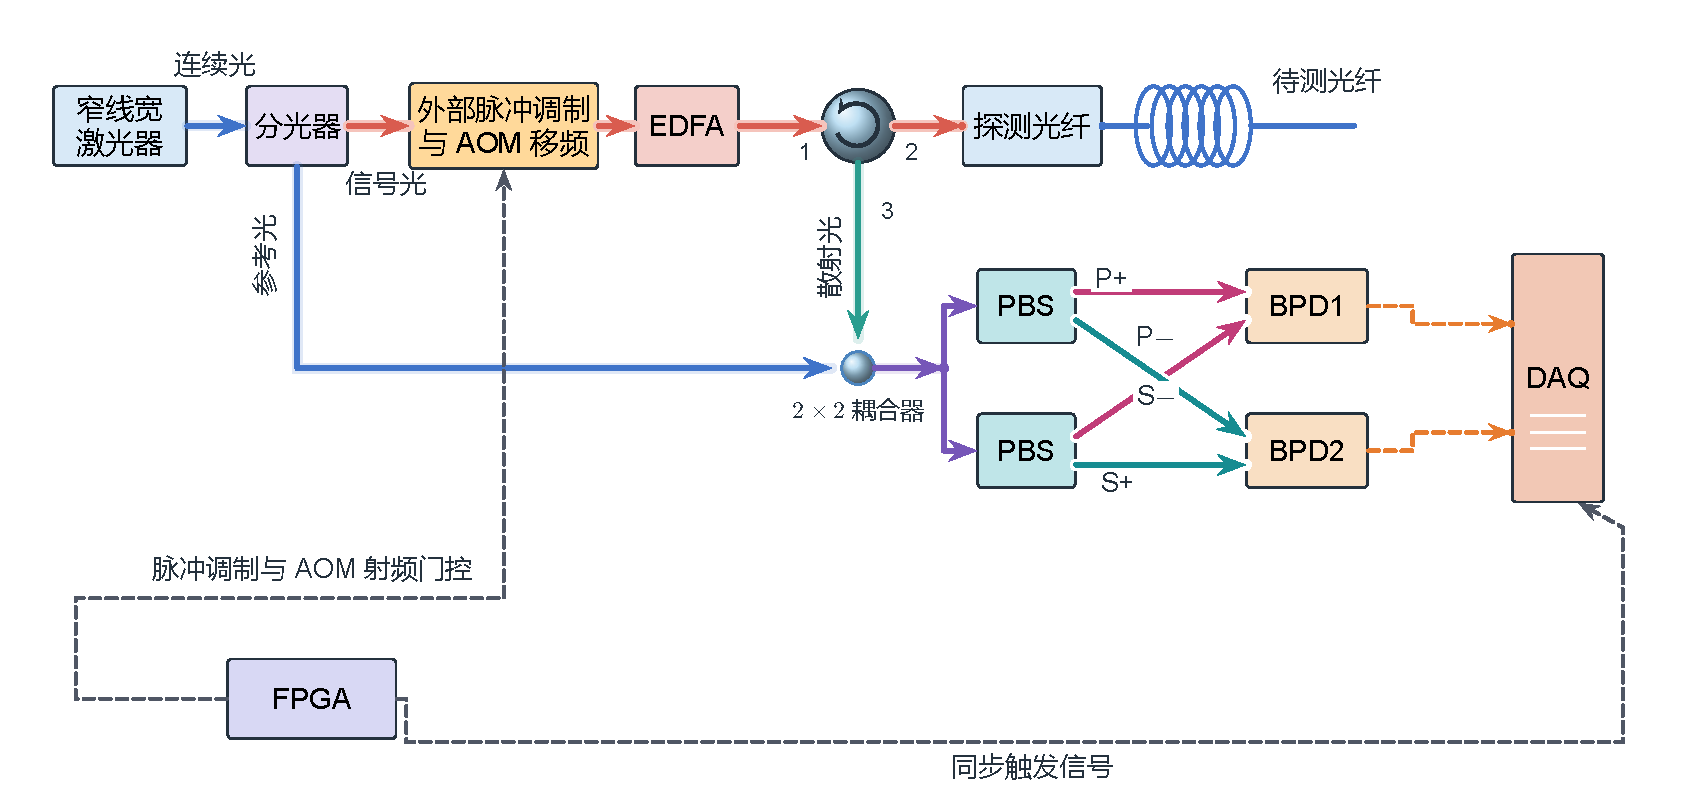
\includegraphics[width=0.96\textwidth]{images/chap3_traditional_proposed_architectures.pdf}
  \caption{传统EDFA分立式偏振分集外差DAS光路}
  \label{fig:chap3_traditional_edfa_architecture}
\end{figure}

与传统方案相比，本文采用双输出ECL--SOA激光器直接提供两条光支路：SOA端输出经光功率放大和电流门控形成脉冲信号光，LD端输出未经SOA放大的连续参考光；脉冲信号光经AOM移频和环形器进入传感光纤，发射链路无EDFA。本文搭建的分立式偏振分集外差DAS光路如图\ref{fig:chap3_das_system}所示，系统由ECL--SOA脉冲发射与传感光路、偏振分集平衡接收链路以及FPGA--DAQ同步控制链路组成。除双输出ECL--SOA激光器外，AOM、环形器、耦合器、PBS和BPD均作为独立器件在实验平台上连接，该系统作为后续评价一体化收发模组的分立光路基线。

图\ref{fig:chap3_traditional_edfa_architecture}和图\ref{fig:chap3_das_system}采用一致的图形表达：红色表示脉冲信号光，蓝色表示参考光，绿色表示瑞利散射回波，紫色表示参考光与回波合束后的光路，品红色和青色分别表示PBS分离出的P、S偏振分量；虚线表示光电探测后的电信号与控制信号。两图分别展示传统EDFA光路和本文ECL--SOA光路。

表\ref{tab:traditional_proposed_architecture}进一步归纳两种光路在发射与接收链路上的结构差异，重点比较双输出ECL--SOA与传统“外部调制器+EDFA”发射架构的实现方式。EDFA与SOA的器件特性及选型依据已在第\ref{sec:edfa_soa_selection}节讨论。

\begin{table}[htbp]
  \centering
  \caption{传统EDFA光路与本文ECL--SOA光路的架构差异}
  \label{tab:traditional_proposed_architecture}
  \renewcommand{\arraystretch}{1.25}
  \small
  \begin{tabular}{p{0.18\textwidth}p{0.35\textwidth}p{0.35\textwidth}}
    \toprule
    比较维度 & 传统EDFA分立光路 & 本文ECL--SOA光路 \\
    \midrule
    激光与分支 & 单输出窄线宽激光器经分光器形成信号光和参考光支路 & 双输出ECL--SOA直接提供SOA端信号光和LD端参考光 \\
    脉冲形成 & 由外部电光调制器或AOM形成探测脉冲 & 由SOA注入电流门控形成探测脉冲 \\
    光功率放大 & 外置EDFA对已形成的探测脉冲进行放大 & 封装内SOA同时承担光功率放大与脉冲形成，发射链路无EDFA \\
    移频与传感 & 信号光经AOM移频、EDFA放大后由环形器进入传感光纤 & SOA端脉冲光经AOM移频后由环形器进入传感光纤 \\
    参考与接收 & 分光得到的参考光与瑞利回波合束后进行相干探测 & LD端连续参考光与瑞利回波合束后进行偏振分集平衡探测 \\
    工程实现 & 多个独立发射器件及光纤连接，结构便于调整但链路较长 & 发射核心紧凑，可进一步按同一拓扑实现为分立系统或集成模组 \\
    \bottomrule
  \end{tabular}
\end{table}

图\ref{fig:chap3_traditional_edfa_architecture}、图\ref{fig:chap3_das_system}及表\ref{tab:traditional_proposed_architecture}用于光路架构比较，即传统EDFA光路与本文ECL--SOA光路的对比，二者的差异在于发射器件和脉冲形成方式。第\ref{sec:chap3_hardware_comparison}节及第4章用于集成效果比较，在尽可能保持ECL工作点、SOA驱动、AOM射频、传感光纤、BPD工作状态、DAQ触发及数字处理流程一致的条件下，评价自搭建分立系统D与集成模组M在器件布置、连接长度、封装和接口形式上造成的变化。

自搭建分立光路工作时，FPGA产生器件调制信号并向DAQ提供同步触发，使光脉冲发射、瑞利回波到达和数据采集具有统一的时间基准。激光器SOA输出端的脉冲信号光经80~MHz AOM移频后进入传感光路，LD输出端的连续参考光则绕过AOM和待测光纤，直接送往接收端作为本振光。传感链路返回的瑞利散射光与参考光在$2\times2$光耦合器中发生干涉，其两路互补输出再经偏振分集和平衡探测转换为电信号，最终由DAQ同步采集。集成光路保持上述功能关系，但将相应光电器件及内部连接固化在DAS一体化收发模组中，具体实现见第3.5节。

\subsection{集成SOA的ECL激光器脉冲发射与传感光路}

脉冲信号光由集成SOA的ECL激光器的SOA输出端输出后，首先通过标称驱动频率为80~MHz的AOM。AOM一方面在一阶衍射条件下为信号光引入光频移，另一方面与SOA共同限定进入传感光纤的有效脉冲窗口。移频后的探测脉冲由光环形器1端口输入、2端口输出，并注入由探测光纤和待测光纤构成的传感链路。光脉冲沿光纤传播过程中产生的瑞利后向散射光由2端口返回环形器，再从3端口导向接收链路，从而实现发射光与回波光的空间分离。本文搭建的ECL--SOA分立式偏振分集外差DAS系统整体光路如图\ref{fig:chap3_das_system}所示。

\begin{figure}[htbp]
  \centering
  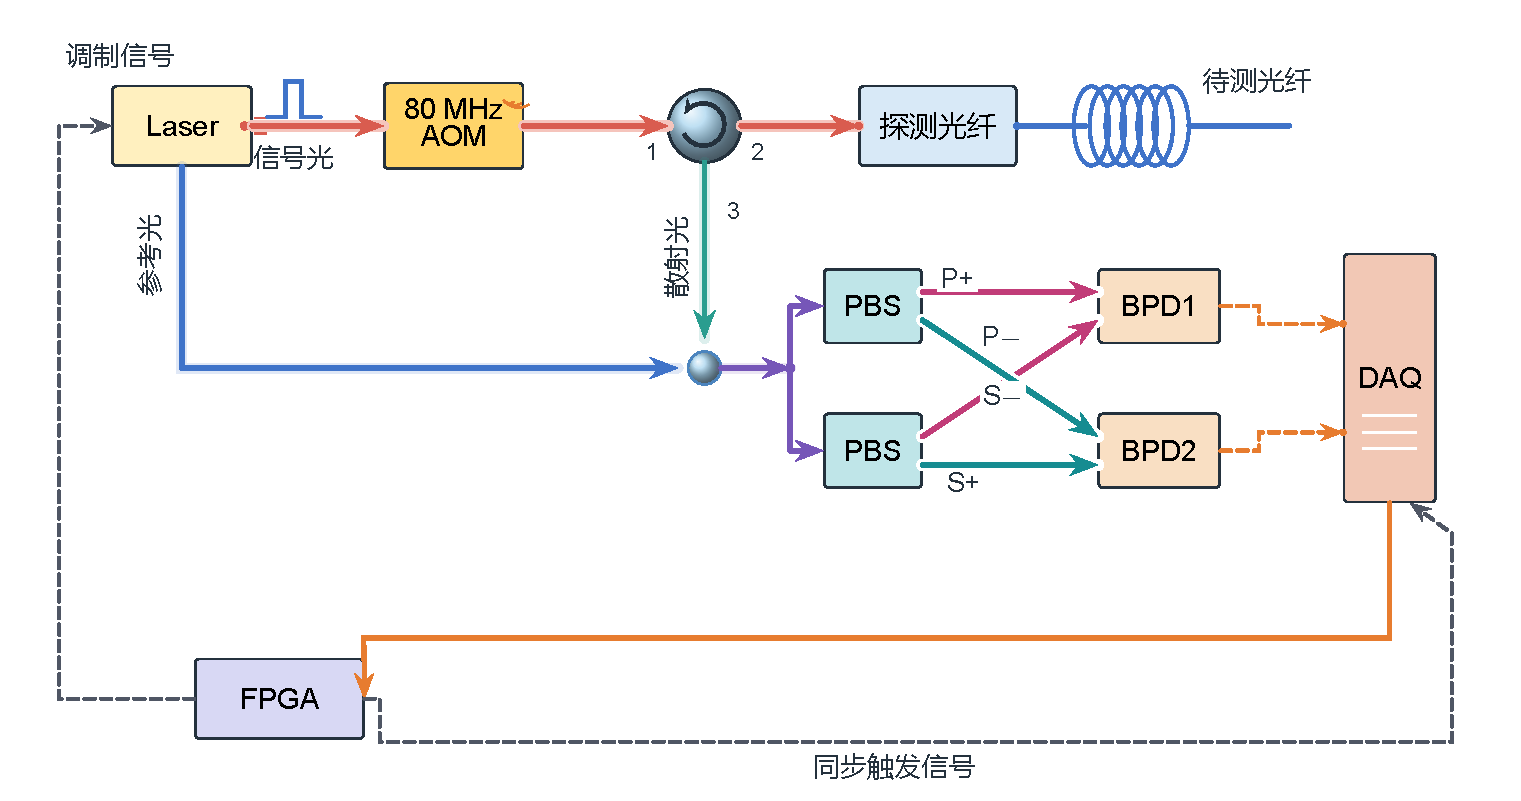
\includegraphics[width=0.98\textwidth]{images/chap3_das_system_schematic_color.pdf}
  \caption{本文搭建的ECL--SOA分立式偏振分集DAS光路}
  \label{fig:chap3_das_system}
\end{figure}

LD输出端的参考光支路不经过SOA、AOM和传感光纤，因而保留激光器的连续载频；SOA输出端的信号光支路经放大、门控和AOM移频后，其瑞利回波与参考光之间形成外差拍频。依据第二章式\eqref{eq:aom_shift}和式\eqref{eq:bpd}，在忽略射频频率误差、采样时钟误差及动态相位扰动的理想条件下，接收拍频应位于$f_b\approx f_A=80~\mathrm{MHz}$附近。该关系只给出系统的标称中频，实际拍频仍可能受到AOM驱动、集成SOA的ECL激光器工作状态、光路时延、环境温度和采样窗口等因素影响。因此，后续对拍频变化的分析将以实测频谱和受控变量实验为依据，而不由AOM标称频率直接替代测量结果。

\subsection{AOM所在支路的选择与依据}

\subsection{偏振分集平衡接收与同步采集}

瑞利散射光与参考光进入$2\times2$光耦合器后形成两路相位互补的干涉输出，两路输出分别送入PBS，并被分解为P、S两个正交偏振分量。其中，P+与P$-$接入BPD1的两个光输入端，S+与S$-$接入BPD2的两个光输入端。两个BPD分别对同一偏振方向上的互补光信号进行差分探测，在理想匹配条件下抑制直流项和共模强度噪声，同时保留包含瑞利散射相位信息的外差拍频项。由此获得的P、S双偏振电信号为后续偏振衰落抑制和相位解调提供两路互补观测量。

BPD1和BPD2的输出分别接入DAQ的两个采集通道。FPGA向集成SOA的ECL激光器输出调制信号，并通过同步触发连接使DAQ采样窗口与光脉冲发射保持确定的时间关系；DAQ与FPGA之间的控制连接用于实现两者的协同工作。本节给出系统的物理光路、端口连接和信号流向；SOA、AOM与DAQ之间的提前建立时间、延迟保持时间及采样窗口配置将在第\ref{sec:chap3_timing}节结合实测脉冲与拍频结果确定，双偏振电信号的偏置、增益、I/Q方向和时延标定见第\ref{sec:chap4_channel_calibration}节。

\section{集成SOA的ECL激光器工作特性及其对拍频信号的影响}

\subsection{SOA驱动电流与输出脉冲特性}

为确定集成SOA的ECL激光器发射链路的可用驱动范围，首先直接测试SOA脉冲电流与输出脉冲之间的关系。实验采用FL-1S型集成SOA的ECL激光器，该器件为内部集成ECL与SOA的ECL激光器，中心波长为1550~nm，静态线宽小于3~kHz。测试期间，ECL驱动电流固定为200~mA，TEC温度固定为30~$^\circ$C，SOA关断阶段施加$-5$~V反向偏置；电脉冲宽度和重复频率分别设为100~ns和2~kHz。SOA脉冲电流由200~mA增加至2000~mA，步进为100~mA。光路中的可调光衰减器在完成设定后保持不变，固定衰减量为42~dB；衰减后的光信号由直流耦合、带宽500~MHz、跨阻增益约11~kV/W的BPD1探测，其单端输出由HDO~4804示波器记录。原始波形的采样时间间隔为20~ns，每个电流点截取399个完整脉冲进行统计。

考虑到SOA驱动板的直流电流输出上限为0.6~A，而脉冲电流输出范围可达到2~A，本文采用“低电流直接测量、高电流探测器换算”的方式统一获得峰值光功率。在200--600~mA范围内，使用JW8103A光功率计对各电流点进行5次直接测量，并与同轮测试所得BPD峰值电压建立对应关系。经确认，BPD在本实验覆盖的高电压范围内保持线性。对25组功率--电压数据进行最小二乘拟合，得到
\begin{equation}
  P_{\mathrm{peak}}=0.5153V_{\mathrm{peak}}+4.990,
  \qquad V_{\mathrm{peak}}[\mathrm{mV}],\;P_{\mathrm{peak}}[\mathrm{mW}],
  \label{eq:soa_power_calibration}
\end{equation}
拟合决定系数$R^2=0.9965$，均方根误差为2.38~mW。随后利用式\eqref{eq:soa_power_calibration}将700--2000~mA范围内的BPD峰值电压换算为SOA峰值光功率。为避免混淆，图\ref{fig:chap3_soa_current_characterization}(c)分别以实心圆和空心方块表示功率计直接测量值与BPD标定换算值；误差棒为5轮重复扫描的标准差，浅色带表示标定均值的95\%置信区间。

\begin{figure}[htbp]
  \centering
  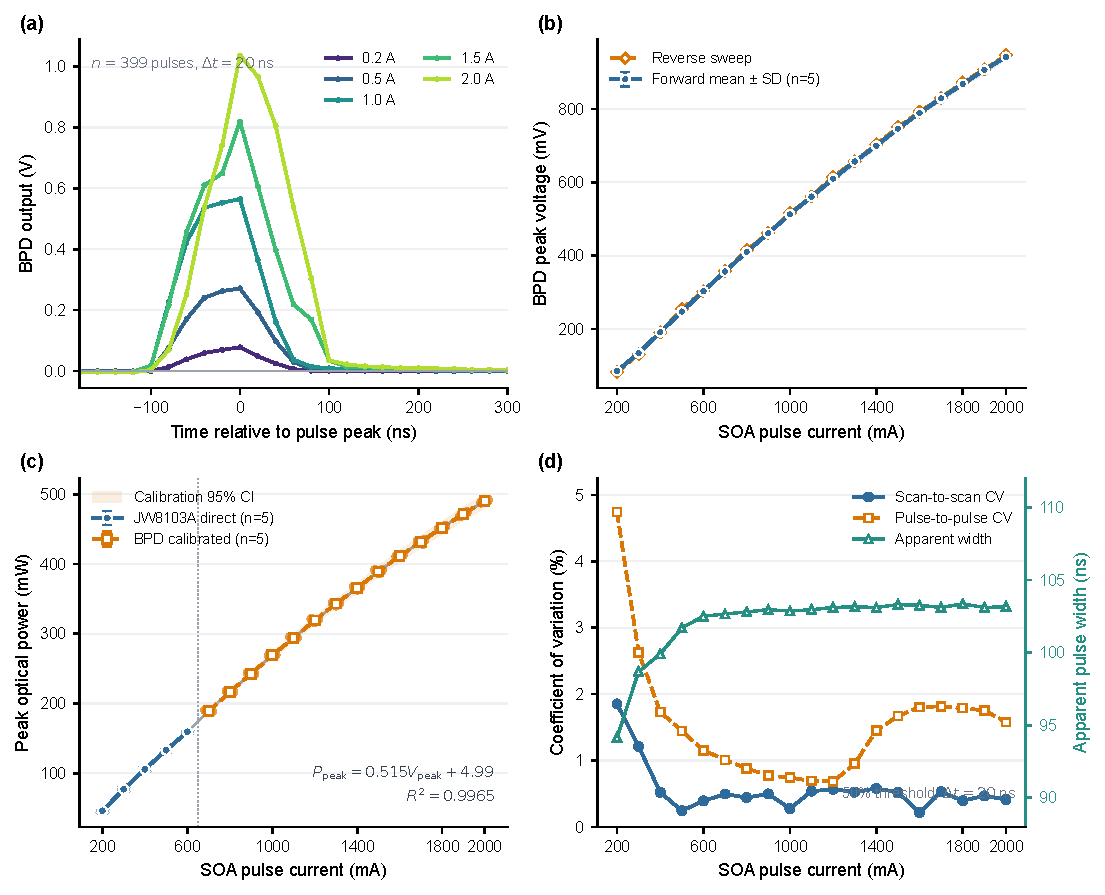
\includegraphics[width=\textwidth]{images/chap3_soa_current_characterization.pdf}
  \caption[不同SOA脉冲电流下的输出脉冲与重复性表征]{不同SOA脉冲电流下的输出脉冲与重复性表征：（a）输出脉冲平均波形；（b）5轮正向扫描的BPD峰值电压及反向扫描结果；（c）峰值光功率，光功率计直测与BPD标定换算；（d）跨轮与脉冲间变异系数及50\%阈值表观脉宽。}
  \label{fig:chap3_soa_current_characterization}
\end{figure}

由图\ref{fig:chap3_soa_current_characterization}(a)和图\ref{fig:chap3_soa_current_characterization}(b)可见，随SOA脉冲电流升高，输出脉冲峰值持续增大，平均BPD峰值电压由200~mA时的86.04~mV增至2000~mA时的941.55~mV。在5轮正向扫描中，各电流点的跨轮变异系数为0.22\%--1.85\%；反向扫描相对于正向均值的平均绝对偏差为0.80\%，最大绝对偏差为3.98\%，且偏差未随电流升高而持续增大。上述结果表明，在本次测试时长和散热条件下，0.2--2.0~A脉冲驱动范围内的峰值输出具有较好的扫描重复性。

峰值光功率结果如图\ref{fig:chap3_soa_current_characterization}(c)所示。200~mA和600~mA下的直接测量结果分别为46.03~mW和159.42~mW；经标定换算，700~mA和2000~mA下的峰值光功率分别为189.11~mW和490.16~mW。功率随驱动电流单调增加，但相邻100~mA电流步进对应的功率增量总体由低电流区的约30~mW逐渐减小至高电流区的约20~mW，呈现边际增益下降趋势。这一现象与SOA在大信号条件下可能出现的增益压缩特征相符\cite{sobhanan2022soa,connelly2023dynamic}，但现有数据尚不能将其单独归因于载流子增益压缩、热效应或驱动波形变化。

图\ref{fig:chap3_soa_current_characterization}(d)进一步给出了脉冲间稳定性。全电流范围内，单个电流点的脉冲峰值变异系数为0.68\%--4.74\%，其中200~mA点因信号幅度较低而具有最大的相对波动；当电流不低于400~mA时，该指标不超过1.82\%。50\%阈值法得到的表观脉宽位于94.14--103.36~ns，未观察到随峰值功率增长而出现的大幅展宽。需要指出的是，20~ns采样间隔限制了对上升沿、下降沿及数纳秒脉宽差异的分辨能力，因此本组数据仅支持“脉冲宽度维持在约100~ns量级”的结论。综合峰值功率、跨轮重复性和脉冲间稳定性，SOA脉冲电流可作为发射功率的有效控制量；后续工作点仍需结合关断消光、拍频信号质量及SOA--AOM--DAQ时序匹配共同确定，而不能仅按峰值功率最大化选择。

\subsection{SOA关断反向偏置与静态消光特性}

SOA关断期间的残余连续光会在相邻探测脉冲之间持续进入传感光纤，有限消光比还可能增加相干噪声并降低$\varphi$-OTDR的测量性能\cite{ren2016extinction}。为定量评价关断反向偏置的作用，在ECL驱动电流200~mA、TEC温度30~$^\circ$C和SOA导通脉冲电流800~mA条件下，将SOA关断偏压依次设置为0、$-1$、$-2$、$-3$、$-4$和$-5$~V。漏光测试时关闭SOA脉冲驱动，使SOA持续保持对应关断偏压，同时维持ECL工作状态不变。采用JW8103A高速光功率计在1550~nm下直接测量功率；测试光路不接入EDFA，并移除前述42~dB光衰减器。导通脉冲峰值功率与关断漏光功率均在同一光学参考面测得。

为避免将功率计零偏和环境背景计入SOA漏光，每个偏压点均配对记录关闭输入激光时的暗态读数$P_{\mathrm{dark}}$，净静态漏光功率及静态消光比分别定义为
\begin{align}
  P_{\mathrm{leak}}&=P_{\mathrm{meter}}-P_{\mathrm{dark}},\
  ER_{\mathrm{static}}&=10\log_{10}\!\left(
  \frac{P_{\mathrm{on,peak}}}{P_{\mathrm{leak}}}
  \right),
  \label{eq:soa_static_extinction}
\end{align}
其中，$P_{\mathrm{meter}}$为SOA持续关断状态下的功率计原始读数，$P_{\mathrm{on,peak}}$为同轮测试中800~mA脉冲驱动下直接测得的峰值功率。实验共完成5轮0至$-5$~V正向扫描和1轮$-5$至0~V反向扫描。该设计既用于评价重复性，也用于检查固定扫描方向导致的时间漂移或回程差异。

\begin{figure}[htbp]
  \centering
  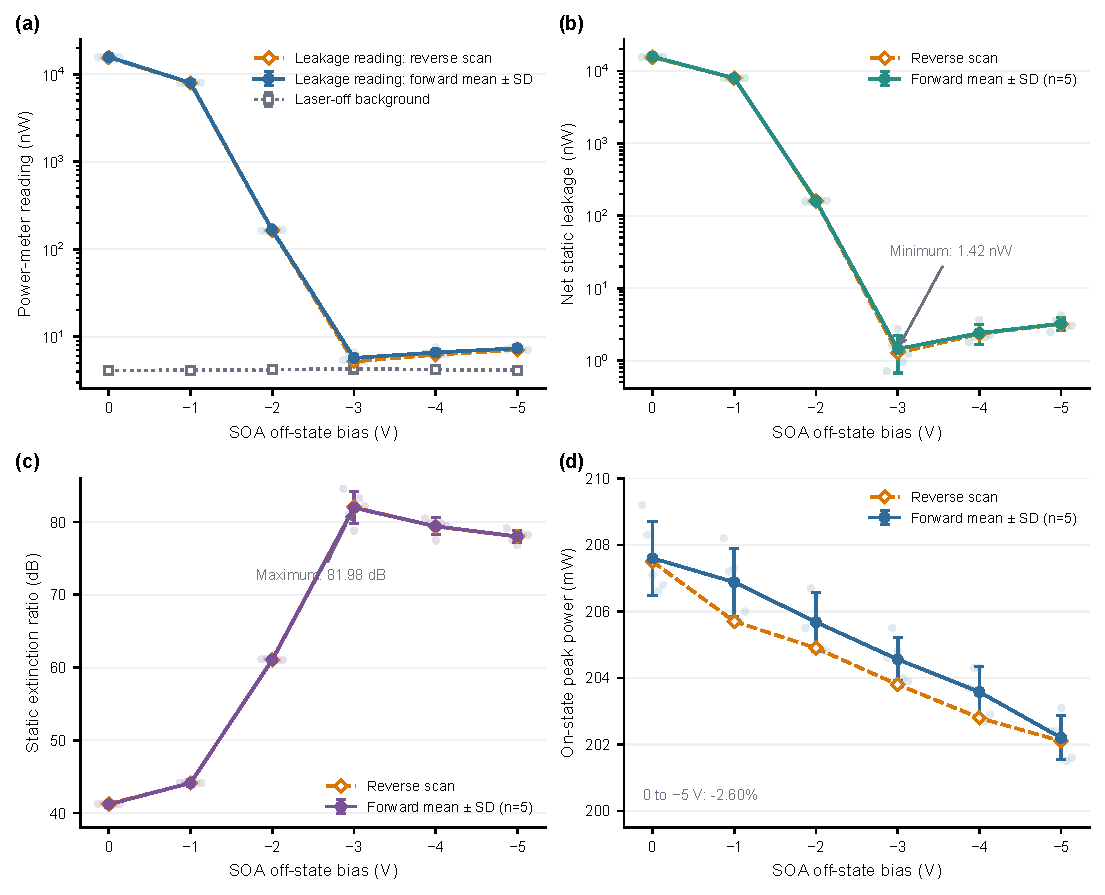
\includegraphics[width=\textwidth]{images/chap3_soa_off_bias_extinction.pdf}
  \caption[不同SOA关断反向偏压下的静态漏光与消光特性]{不同SOA关断反向偏压下的静态漏光与消光特性：（a）漏光原始读数与暗态背景；（b）扣除暗态背景后的净漏光功率；（c）静态消光比；（d）800~mA导通脉冲峰值功率。浅色散点、实线误差棒与空心菱形虚线分别表示5轮正向扫描的单次结果、均值与标准差及反向扫描结果。}
  \label{fig:chap3_soa_off_bias_extinction}
\end{figure}

如图\ref{fig:chap3_soa_off_bias_extinction}(a)所示，全部36组暗态读数的均值为4.134~nW，标准差为0.248~nW。配对扣除暗态后，0、$-1$和$-2$~V下的净静态漏光功率分别为15.718~$\upmu$W、7.967~$\upmu$W和161.17~nW；当反向偏压增加至$-3$~V时，净静态漏光降至$(1.417\pm0.694)$~nW。对应静态消光比由0~V时的$(41.21\pm0.10)$~dB增至$-2$~V时的$(61.06\pm0.10)$~dB，并在$-3$~V达到$(81.98\pm1.97)$~dB。上述均值和标准差由5轮正向扫描与1轮反向扫描共同计算，且$-3$~V下6次净漏光结果均高于其各自配对的暗态读数。

反向扫描结果与正向扫描的变化趋势一致。各偏压点反向扫描所得静态消光比与正向均值的最大绝对差为0.068~dB，导通峰值功率的最大相对差为0.57\%。净漏光功率的最大相对差出现在$-3$~V，为11.73\%，但其绝对差仅为0.170~nW；这是由于扣底噪后的净漏光已接近nW量级，较小的绝对变化会被相对量放大。因此，正、反向扫描对照未显示足以改变静态消光比判断的明显回程偏差。

继续增大反向偏压并未进一步降低静态漏光：$-4$和$-5$~V下的净漏光分别回升至$(2.389\pm0.647)$~nW和$(3.235\pm0.580)$~nW，对应静态消光比分别为$(79.41\pm1.03)$~dB和$(78.02\pm0.76)$~dB。与此同时，800~mA导通脉冲峰值功率由0~V时的207.58~mW缓慢降至$-5$~V时的202.18~mW，降幅为2.60\%。该非单调变化在正、反向扫描中均可重复观察，说明其具有重复性；其微观机制可能同时涉及器件反向偏置特性、驱动状态切换和测量零点变化，需要结合动态测量进一步辨识。

本组结果表明，在800~mA导通电流下，施加反向关断偏压可使静态消光比提高约40~dB，其中$-3$~V附近获得本实验条件下最低的静态漏光。功率计测量反映SOA持续处于关断偏压时的静态状态，脉冲关断边沿、载流子恢复和相邻脉冲间瞬态漏光需要通过动态测量表征。因此，$-3$~V是本组静态测试的最优点；实际系统工作点还需结合动态脉冲完整性、拍频质量和时序裕量评价图\ref{fig:chap3_soa_current_characterization}采用的$-5$~V条件。

\subsection{SOA工作状态对拍频信号的影响}

\section{SOA--AOM--DAQ协同门控方法}
\label{sec:chap3_timing}

\subsection{协同门控的必要性与时序定义}

\subsection{三种门控策略与对照实验设计}

三种AOM射频策略及其与SOA光脉冲、DAQ采样窗口之间的关系如图\ref{fig:chap3_coordinated_timing}所示。连续射频策略使AOM长期处于稳定衍射状态，可作为光脉冲完整性的参照，但会持续产生射频功耗和温升；命令边沿简单同步策略同时开启SOA与AOM射频，未补偿声场传播和建立时间，稳定衍射窗口可能与有效光脉冲不能完全重合；预补偿协同门控则使AOM射频相对于SOA提前开启并延迟关闭，以覆盖完整光脉冲，同时由统一触发确定DAQ有效采样窗口。

\begin{figure}[htbp]
  \centering
  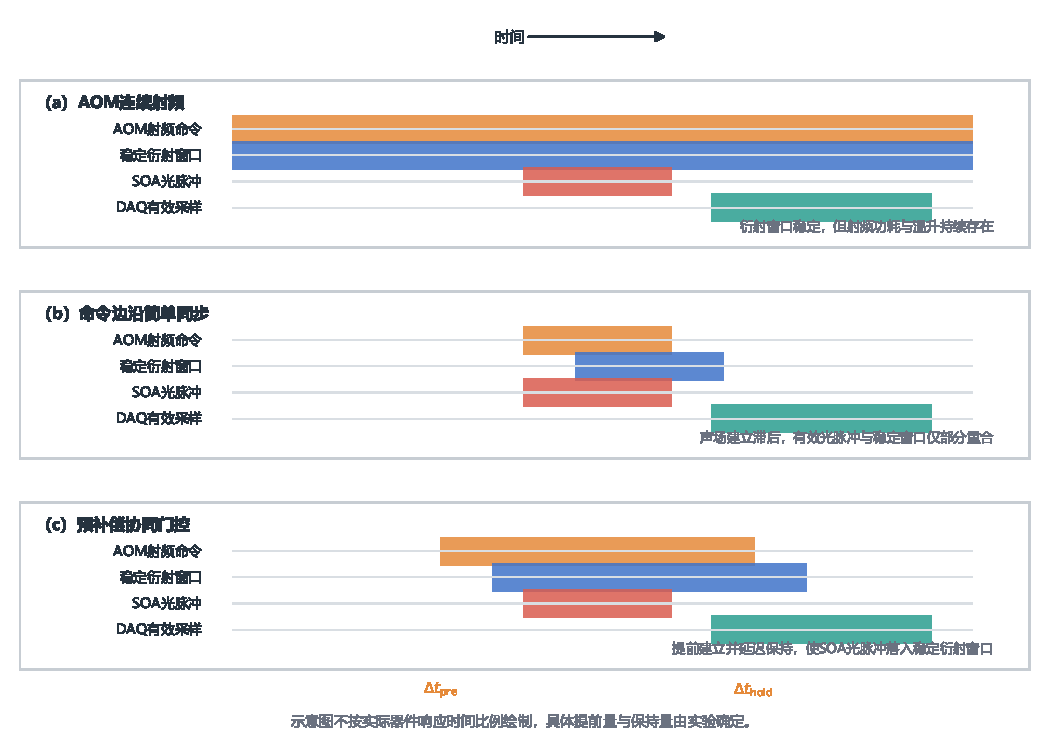
\includegraphics[width=0.96\textwidth]{images/chap3_coordinated_timing.pdf}
  \caption{连续射频、命令边沿简单同步与预补偿协同门控的时序对比}
  \label{fig:chap3_coordinated_timing}
\end{figure}

图中时序说明三种策略和$\Delta t_{\mathrm{pre}}$、$\Delta t_{\mathrm{hold}}$的定义，图示比例不代表实际器件响应时间。具体提前建立时间、延迟保持时间和DAQ采样延迟由AOM衍射光响应、SOA输出脉冲和外差拍频的同步测量确定。

\subsection{门控策略对脉冲、功耗与温升的影响}

\subsection{门控策略对拍频与相位稳定性的影响}

\section{DAS一体化收发模组设计与实现}

\subsection{模组功能需求与总体方案}

\subsection{光路拓扑与器件布局}

\subsection{接口、封装、散热与屏蔽设计}

\subsection{模组装调与实现}

\section{模组光电性能测试}
\label{sec:chap3_hardware_comparison}

\subsection{输出光功率与总插入损耗测试}

\subsection{收发隔离与内部串扰测试}

\subsection{双偏振通道一致性与拍频质量}

\subsection{硬件热稳定性与输出重复性}

\section{本章小结}
